% Presentation: Predicting New-User Engagement on Zindi
% Compile: pdflatex slides.tex (twice). Figures are produced by ../notebook/zindi_engagement.ipynb into ../figures/.
\RequirePackage{silence}
\WarningFilter{beamerthememetropolis}{You need to compile with XeLaTeX or LuaLaTeX}  % Fira loaded through the pdflatex package below
\documentclass[aspectratio=169,10pt]{beamer}
\usetheme[numbering=none,block=fill,sectionpage=none]{metropolis}
\usepackage[T1]{fontenc}
\usepackage[utf8]{inputenc}
\usepackage[sfdefault,lining]{FiraSans}             % same font family as the figures
\usepackage[scale=0.88]{FiraMono}
\usepackage{booktabs,amsmath,amssymb,graphicx,array,tikz}
\usepackage[most]{tcolorbox}
\graphicspath{{../figures/}}
\setlength{\parskip}{0pt}

%---------------------------------------------------------------- colours (same palette as the figures)
\definecolor{ink}{HTML}{1D2B3A}
\definecolor{accent}{HTML}{3A6EA5}
\definecolor{warn}{HTML}{C0504D}
\definecolor{soft}{HTML}{EEF3F9}
\definecolor{muted}{HTML}{7A8794}
\setbeamercolor{normal text}{fg=ink,bg=white}
\setbeamercolor{background canvas}{bg=white}
\setbeamercolor{alerted text}{fg=warn}
\setbeamercolor{example text}{fg=accent}
\setbeamercolor{block title}{fg=accent,bg=soft}
\setbeamercolor{block body}{fg=ink,bg=soft}
\setbeamerfont{block title}{series=\bfseries,size=\normalsize}
\setbeamercolor{standout}{fg=white,bg=ink}

%---------------------------------------------------------------- lists
\setbeamertemplate{itemize item}{\raisebox{0.2ex}{\color{accent}\rule{0.42em}{0.42em}}}
\setbeamertemplate{itemize subitem}{\raisebox{0.25ex}{\color{muted}\rule{0.32em}{0.32em}}}
\setbeamertemplate{enumerate item}{\color{accent}\bfseries\insertenumlabel.}

%---------------------------------------------------------------- frame title: section kicker + title + rubric tag + progress line
\makeatletter
\newcommand{\rubric}[1]{\gdef\zz@rubric{#1}}            % rubric tag, shown at the top right of the frame title
\gdef\zz@rubric{}
\newcommand{\zz@kicker}{\ifnum\value{section}>0 \insertsectionnumber\enspace\textbar\enspace\insertsection\else Overview\fi}
\setbeamertemplate{frametitle}{%
  \gdef\zz@rubric{}%
  \setbox0=\hbox{\usebeamerfont{frametitle}\insertframetitle}%   sets \zz@rubric if the title contains \rubric
  \nointerlineskip
  \begin{tikzpicture}[x=1cm,y=1cm,remember picture]
    \useasboundingbox (0,0) rectangle (0.1,1.42);
    \begin{scope}[overlay,shift={([yshift=-1.48cm]current page.north west)}]
    \fill[accent] (0,0.28) rectangle (0.16,1.22);
    \node[anchor=base west,inner sep=0,text=accent,font=\scriptsize\bfseries] at (0.6,0.98) {\MakeUppercase{\zz@kicker}};
    \node[anchor=base west,inner sep=0,text=ink,font=\Large\bfseries] at (0.6,0.42) {\insertframetitle};
    \ifx\zz@rubric\@empty\else
      \node[anchor=base east,inner sep=2.5pt,rounded corners=2pt,fill=soft,text=accent,font=\scriptsize]
        at (\paperwidth-0.6cm,0.98) {\zz@rubric};
    \fi
    \draw[black!12,line width=0.5pt] (0.6,0.2) -- (\paperwidth-0.6cm,0.2);
    \pgfmathsetlengthmacro{\zz@prog}{(\paperwidth-1.2cm)*\insertframenumber/max(\inserttotalframenumber,1)}
    \fill[accent] (0.6,0.18) rectangle ++(\zz@prog,0.045);
    \end{scope}
  \end{tikzpicture}%
}
\setbeamertemplate{frametitle continuation}{}
\makeatother

%---------------------------------------------------------------- footline: short title, authors, page
\setbeamertemplate{footline}{%
  \hbox to \paperwidth{\hspace{0.6cm}%
    \color{muted}\tiny Zindi new-user engagement\enspace\textbar\enspace Zhiran Zhang \& Haolin Yang\hfill
    \insertframenumber\,/\,\inserttotalframenumber\hspace{0.6cm}}%
  \vspace{2.2mm}}

%---------------------------------------------------------------- section page: big number + chapter list with the current one highlighted
\AtBeginSection{%
  \begin{frame}[plain,noframenumbering]
  \begin{tikzpicture}[remember picture,overlay]
    \fill[soft] (current page.north west) rectangle ([xshift=5.2cm]current page.south west);
    \fill[accent] ([xshift=5.2cm]current page.north west) rectangle ([xshift=5.32cm]current page.south west);
    \node[anchor=east,text=accent,font=\fontsize{64}{64}\selectfont\bfseries]
      at ([xshift=4.6cm,yshift=0.4cm]current page.west) {\ifnum\value{section}<10 0\fi\insertsectionnumber};
  \end{tikzpicture}%
  \hspace*{4.9cm}\begin{minipage}{0.6\paperwidth}\raggedright
    {\color{muted}\footnotesize SECTION \insertsectionnumber}\\[2pt]
    {\Huge\bfseries\color{ink}\insertsectionhead}\\[16pt]
    {\footnotesize\tableofcontents[currentsection,hideallsubsections,sectionstyle=show/shaded]}
  \end{minipage}
  \end{frame}}
\setbeamertemplate{section in toc}{\color{accent}\inserttocsectionnumber.\enspace\color{ink}\inserttocsection}
\setbeamertemplate{section in toc shaded}[default][35]

%---------------------------------------------------------------- helpers
\newcolumntype{L}[1]{>{\raggedright\arraybackslash}p{#1}}
\newcommand{\key}[1]{\begin{block}{}\centering #1\end{block}}
% card: titled box with a coloured top rule
\newtcolorbox{card}[2][]{enhanced,colback=white,colframe=accent,boxrule=0pt,toprule=2pt,arc=0pt,
  left=5pt,right=5pt,top=1pt,bottom=2pt,fonttitle=\bfseries\small,coltitle=accent,colbacktitle=white,
  title={#2},titlerule=0pt,borderline south={0.4pt}{0pt}{black!12},
  fontupper=\small,before upper={\raggedright\let\olditemize\itemize\renewcommand\itemize{\olditemize\setlength{\itemsep}{0pt}}},
  before skip=0pt,after skip=3pt,#1}
\tcbset{red/.style={colframe=warn,coltitle=warn},grey/.style={colframe=muted,coltitle=muted},tight/.style={fontupper=\footnotesize}}
% takeaway: tinted box with a thick left bar
\newtcolorbox{takeaway}[1][accent]{enhanced,colback=soft,colframe=#1,boxrule=0pt,leftrule=3pt,arc=0pt,
  left=6pt,right=6pt,top=3pt,bottom=3pt,fontupper=\small,before upper=\raggedright,before skip=2pt,after skip=2pt}
% source note: where the numbers come from
\newcommand{\src}[1]{\begin{tikzpicture}[remember picture,overlay]
  \node[anchor=south east,inner sep=0,text=muted,font=\tiny] at ([xshift=-0.6cm,yshift=0.62cm]current page.south east) {#1};
\end{tikzpicture}}

\title{Predicting New-User Engagement on Zindi}
\subtitle{Will a user who just signed up still be active in their second month?}
\author{Zhiran Zhang \texorpdfstring{\quad}{, } Haolin Yang}
\institute{ML with Python, Final Project\\ \small Data: Zindi New User Engagement Prediction Challenge}
\date{}

\makeatletter
\setbeamertemplate{title page}{%
  \begin{tikzpicture}[remember picture,overlay]
    \fill[ink] (current page.north west) rectangle ([xshift=0.45cm]current page.south west);
    \fill[accent] ([xshift=0.45cm]current page.north west) rectangle ([xshift=0.6cm]current page.south west);
    \fill[soft] ([yshift=1.9cm]current page.south west) rectangle (current page.south east);
  \end{tikzpicture}%
  \vspace*{0.9cm}
  \begin{minipage}{0.9\textwidth}\raggedright
    {\color{accent}\scriptsize\bfseries ML WITH PYTHON\enspace\textbar\enspace FINAL PROJECT}\\[8pt]
    {\fontsize{24}{28}\selectfont\bfseries\color{ink}\inserttitle}\\[6pt]
    {\large\color{accent}\insertsubtitle}\\[16pt]
    {\color{ink}\insertauthor}\\[4pt]
    {\color{muted}\footnotesize\insertinstitute}
  \end{minipage}}
\makeatother

\begin{document}

%---------------------------------------------------------------- 1
\begin{frame}[plain,noframenumbering]
\titlepage
\end{frame}

%---------------------------------------------------------------- 2
\begin{frame}{Roadmap}
\begin{columns}[T]
\column{0.53\textwidth}
\begin{enumerate}\setlength{\itemsep}{5pt}
  \item Problem: why it matters, how ML helps
  \item Data: load with pandas, time axis, target, X / y
  \item Data preparation
  \item Exploratory analysis (Seaborn)
  \item Validation, metric, models, tuning
  \item Results, impact, conclusions
\end{enumerate}
\column{0.42\textwidth}
\begin{card}{Two label definitions}
The M4 activity log ends on day 22. All models are trained and tested with \textbf{two labels}:
\begin{itemize}
  \item \textbf{A}: active in the whole next month
  \item \textbf{B}: active in days 1--22 of the next month (aligned)
\end{itemize}
\end{card}
\end{columns}
\end{frame}

%================================================================
\section{Problem}

\begin{frame}{The problem and why it matters \rubric{Problem}}
\vspace*{-8pt}
\begin{columns}[T]
\column{0.485\textwidth}
\begin{card}{Context}
\begin{itemize}
  \item Zindi: Africa's largest data-science competition platform, $\approx$12\,k sign-ups in 7 months
  \item Only \textbf{12--21\,\%} of a typical cohort comes back in month 2
\end{itemize}
\end{card}
\begin{card}{Task}
\begin{itemize}
  \item At the end of a user's \textbf{first month}, predict: active in the \textbf{next month}?
  \item Binary classification, minority positive class
\end{itemize}
\end{card}
\column{0.485\textwidth}
\begin{card}{Why it matters}
\begin{itemize}
  \item Acquisition is expensive; month-2 survivors become competitors and hires
  \item Churn is fast: Zindi must act right after month 1
\end{itemize}
\end{card}
\begin{card}[red]{How the model helps}
\begin{itemize}
  \item \textbf{Lower cost}: retention offers only to users who need them
  \item \textbf{Prioritise}: invite likely-engaged users to hackathons
  \item \textbf{Insight}: which behaviours drive retention
\end{itemize}
\end{card}
\end{columns}
\src{Notebook \S1}
\end{frame}

%================================================================
\section{Data and target}

\begin{frame}{Loading the data and recovering the time axis \rubric{Load data, X / y}}
\begin{columns}[c]
\column{0.37\textwidth}
\small
\begin{itemize}\setlength{\itemsep}{3pt}
  \item 8 tables loaded with \texttt{pandas.read\_csv} (Users, UserActivity with 317\,k events, \dots)
  \item Months are \textbf{masked}; sign-up $\times$ activity table is upper-triangular only in the order\\ \textbf{M11 $\to$ M12 $\to$ M1 $\to \dots \to$ M5}
  \item M4 cohort = official test set (M5 activity removed)
\end{itemize}
\begin{takeaway}
$X$: 9\,026 users $\times$ 50 features\\ $y_A$, $y_B$: \texttt{Active} (0/1)
\end{takeaway}
\column{0.61\textwidth}
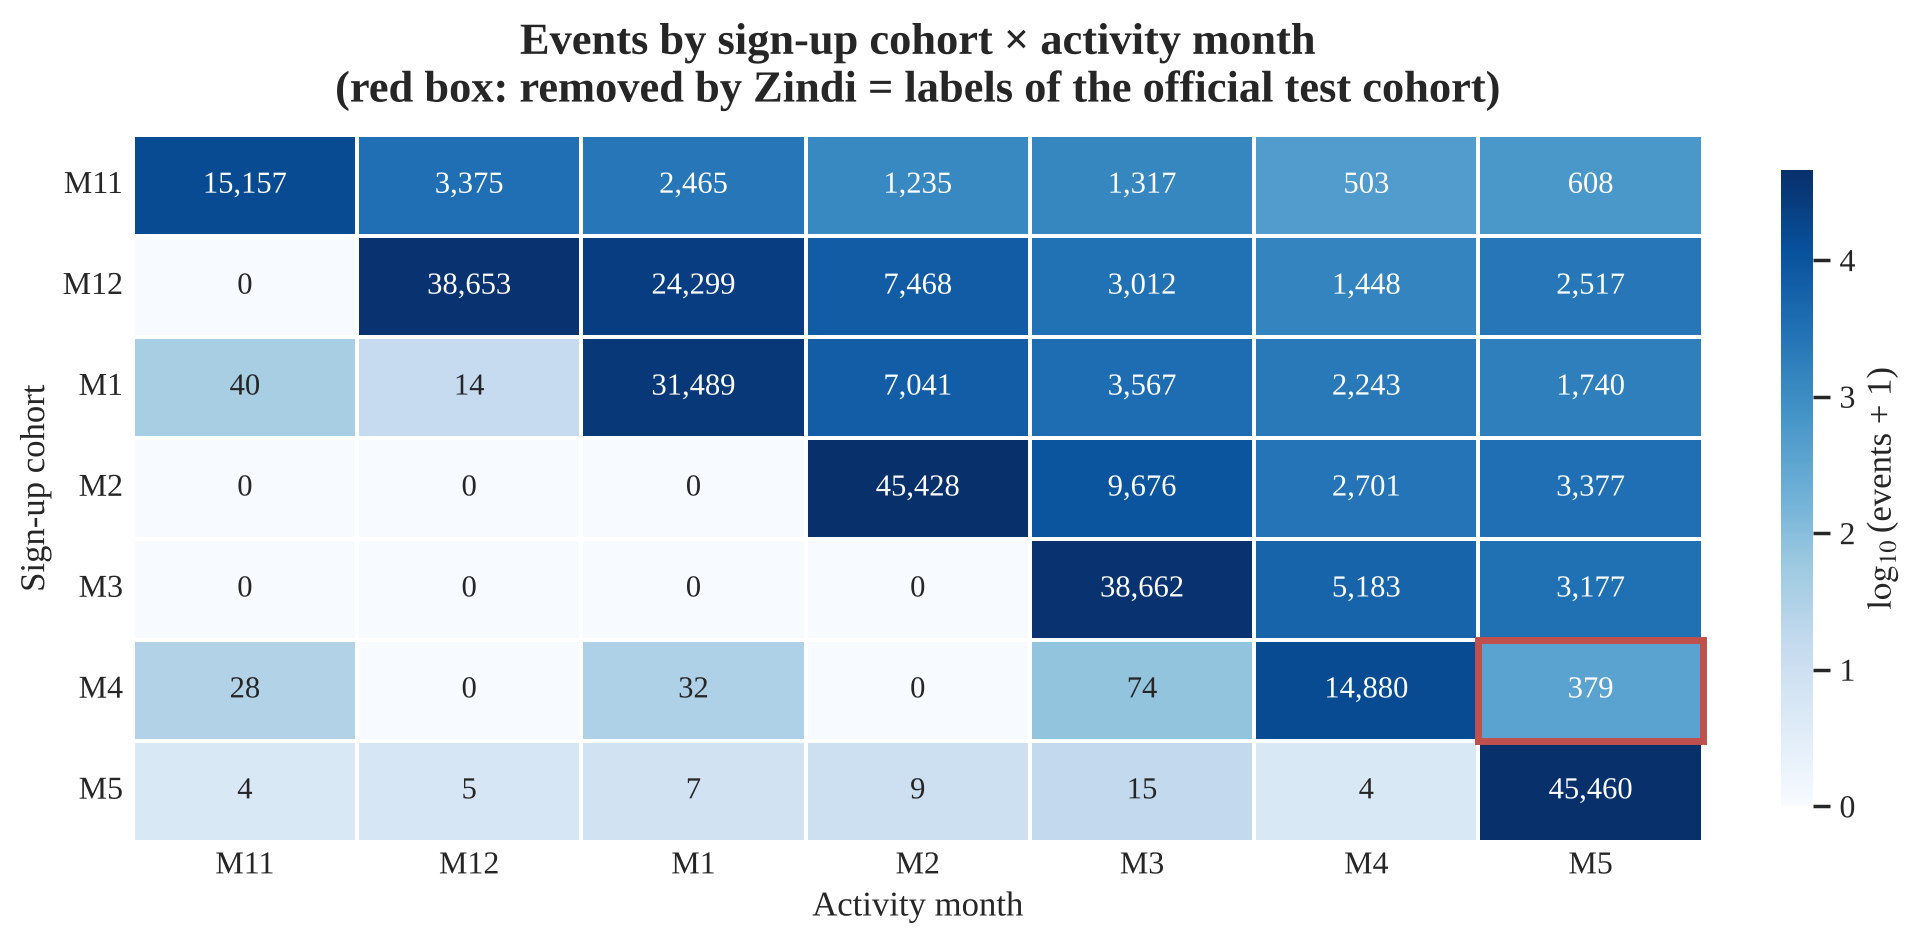
\includegraphics[width=\linewidth]{fig01_time_axis}
\end{columns}
\src{Notebook \S1.1--1.2}
\end{frame}

\begin{frame}{Test on a period later than the training data}
\begin{columns}[c]
\column{0.45\textwidth}
\begin{itemize}\setlength{\itemsep}{4pt}
  \item Time-ordered data $\Rightarrow$ the test set must come \textbf{after} the training data
  \item Labelled cohorts: M11, M12, M1, M2, M3
  \item $\Rightarrow$ the \textbf{latest} one, \textbf{M3}, is our hold-out test cohort
  \item Any other choice trains on the future or wastes a month of data
\end{itemize}
\column{0.5\textwidth}
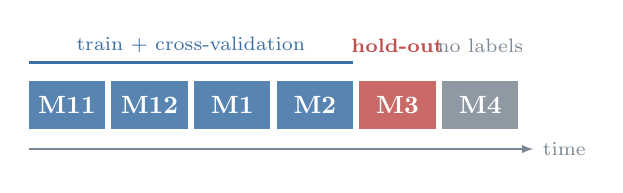
\begin{tikzpicture}[x=1.05cm,y=1cm,font=\small]
  % time line of cohorts with their role
  \foreach \m/\i/\c in {M11/0/accent,M12/1/accent,M1/2/accent,M2/3/accent,M3/4/warn,M4/5/muted}{
    \fill[\c!85] (\i,0) rectangle ++(0.92,0.62);
    \node[text=white,font=\small\bfseries] at (\i+0.46,0.31) {\m};
  }
  \draw[-latex,muted] (0,-0.25) -- (6.1,-0.25) node[right,font=\scriptsize] {time};
  \draw[accent,thick] (0,0.85) -- (3.92,0.85); \node[accent,font=\scriptsize,above] at (1.96,0.85) {train + cross-validation};
  \node[warn,font=\scriptsize\bfseries,above] at (4.46,0.85) {hold-out};
  \node[muted,font=\scriptsize,above] at (5.46,0.85) {no labels};
\end{tikzpicture}\\[10pt]
\small
\begin{tabular}{ll}\toprule
Cohorts & Role\\\midrule
M11, M12, M1, M2 & train + cross-validation\\
\textbf{M3} & \textbf{hold-out test} (scored once)\\
M4 & official test (no labels)\\\bottomrule
\end{tabular}
\end{columns}
\src{Notebook \S1.2}
\end{frame}

\begin{frame}{Truncated labels in the hold-out cohort}
\begin{columns}[c]
\column{0.4\textwidth}
\footnotesize
\begin{tabular}{lc}\toprule
Table & Last day in M4\\\midrule
UserActivity$^*$ & \alert{\textbf{22}}\\
CompetitionPart. & 30\\
Discussion & 30\\\bottomrule
\end{tabular}\\[2pt]
{\scriptsize $^*$page views and clicks, most of the events}
\column{0.56\textwidth}
\small
\begin{itemize}
  \item M3's label is measured in M4
  \item Users returning after day 22 $\to$ labelled \textbf{0}
  \item Normally 8--11\,\% of returners come after day 22; in M3 only \alert{1.6\,\%}
\end{itemize}
\end{columns}
\vspace{4pt}
\centering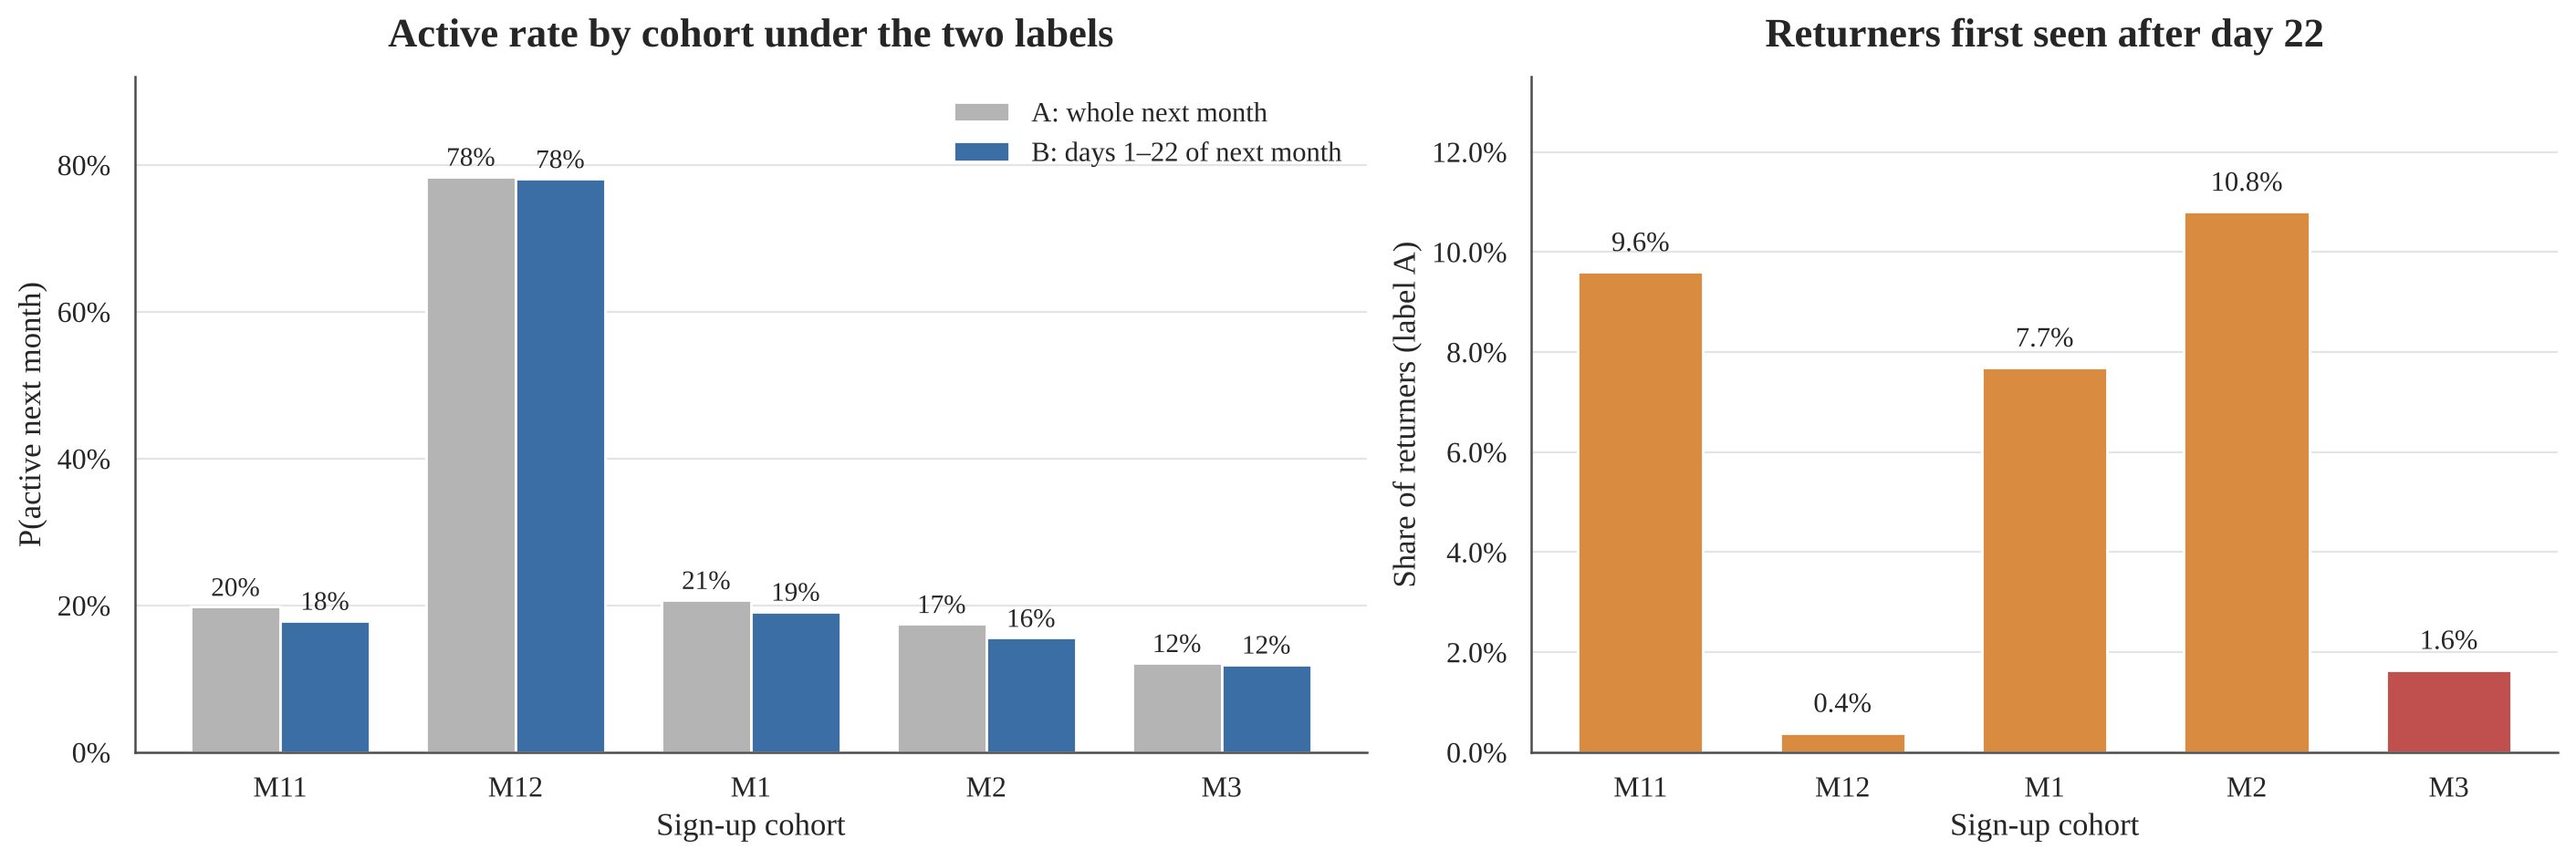
\includegraphics[height=0.47\textheight]{fig02_label_window}
\src{Notebook \S1.3}
\end{frame}

\begin{frame}{Label-definition inconsistency and label B \rubric{Target preprocessing}}
\begin{columns}[T]
\column{0.5\textwidth}
\begin{card}[red,tight]{With a whole-month label (A)}
\begin{itemize}
  \item Training: $y=1$ = ``active in the next $\sim$30 days''
  \item Test (M3): $y=1$ = mostly ``active in the first 22 days''
  \item Features aligned, \alert{labels not aligned}
\end{itemize}
\end{card}
\begin{card}[red,tight]{Consequences}
\begin{itemize}
  \item Biased F1 estimate on M3
  \item Threshold tuned on 17--21\,\% return rates, applied to an artificially low cohort
  \item Lower M3 return rate is partly an artefact of the cutoff
\end{itemize}
\end{card}
\column{0.46\textwidth}
\begin{block}{Label B}
\texttt{Active} = any record in \textbf{days 1--22} of the next month, for \textbf{every} cohort, training and test.
\end{block}
\medskip
Same features, folds and models.\\
We run everything with \textbf{A} (original) and \textbf{B} (aligned) and report both.
\end{columns}
\src{Notebook \S1.3}
\end{frame}

%================================================================
\section{Data preparation}

\begin{frame}{Preparing the dataset \rubric{Preparation}}
\footnotesize
\renewcommand{\arraystretch}{1.25}
\begin{tabular}{L{3.7cm}L{4.3cm}L{4.0cm}}\toprule
\textbf{\color{accent}Issue} & \textbf{\color{accent}What we do} & \textbf{\color{accent}Why}\\\midrule
Multi-table event logs & aggregate per user, \textbf{sign-up month only} & one row per user, no leakage\\
70+ event titles & 18 behaviour families & type of behaviour generalises\\
Country missing (47\,\%) & \texttt{Missing} category + flag & missingness is informative\\
146 countries & top 10 + \texttt{Other}, one-hot & avoids over-fitting rare levels\\
\texttt{FeatureY} codes, \texttt{\textquotedbl{}count 10\textquotedbl} strings & one-hot; parse number, NaN $\to$ 0 & nominal codes; NaN = none\\
Late sign-ups have less time & \texttt{days\_observed}, \texttt{active\_day\_ratio} & normalise by exposure\\\bottomrule
\end{tabular}
\medskip

\begin{takeaway}
\textbf{New features}: recency (\texttt{days\_since\_last}), regularity (\texttt{n\_active\_days}), behaviour counts,
\texttt{joined\_hackathon}, \texttt{n\_new\_comps\_joined}, discussions, profile.
\end{takeaway}
\src{Notebook \S2}
\end{frame}

%================================================================
\section{Exploratory analysis}

\begin{frame}{EDA 1: retention by cohort \rubric{EDA}}
\centering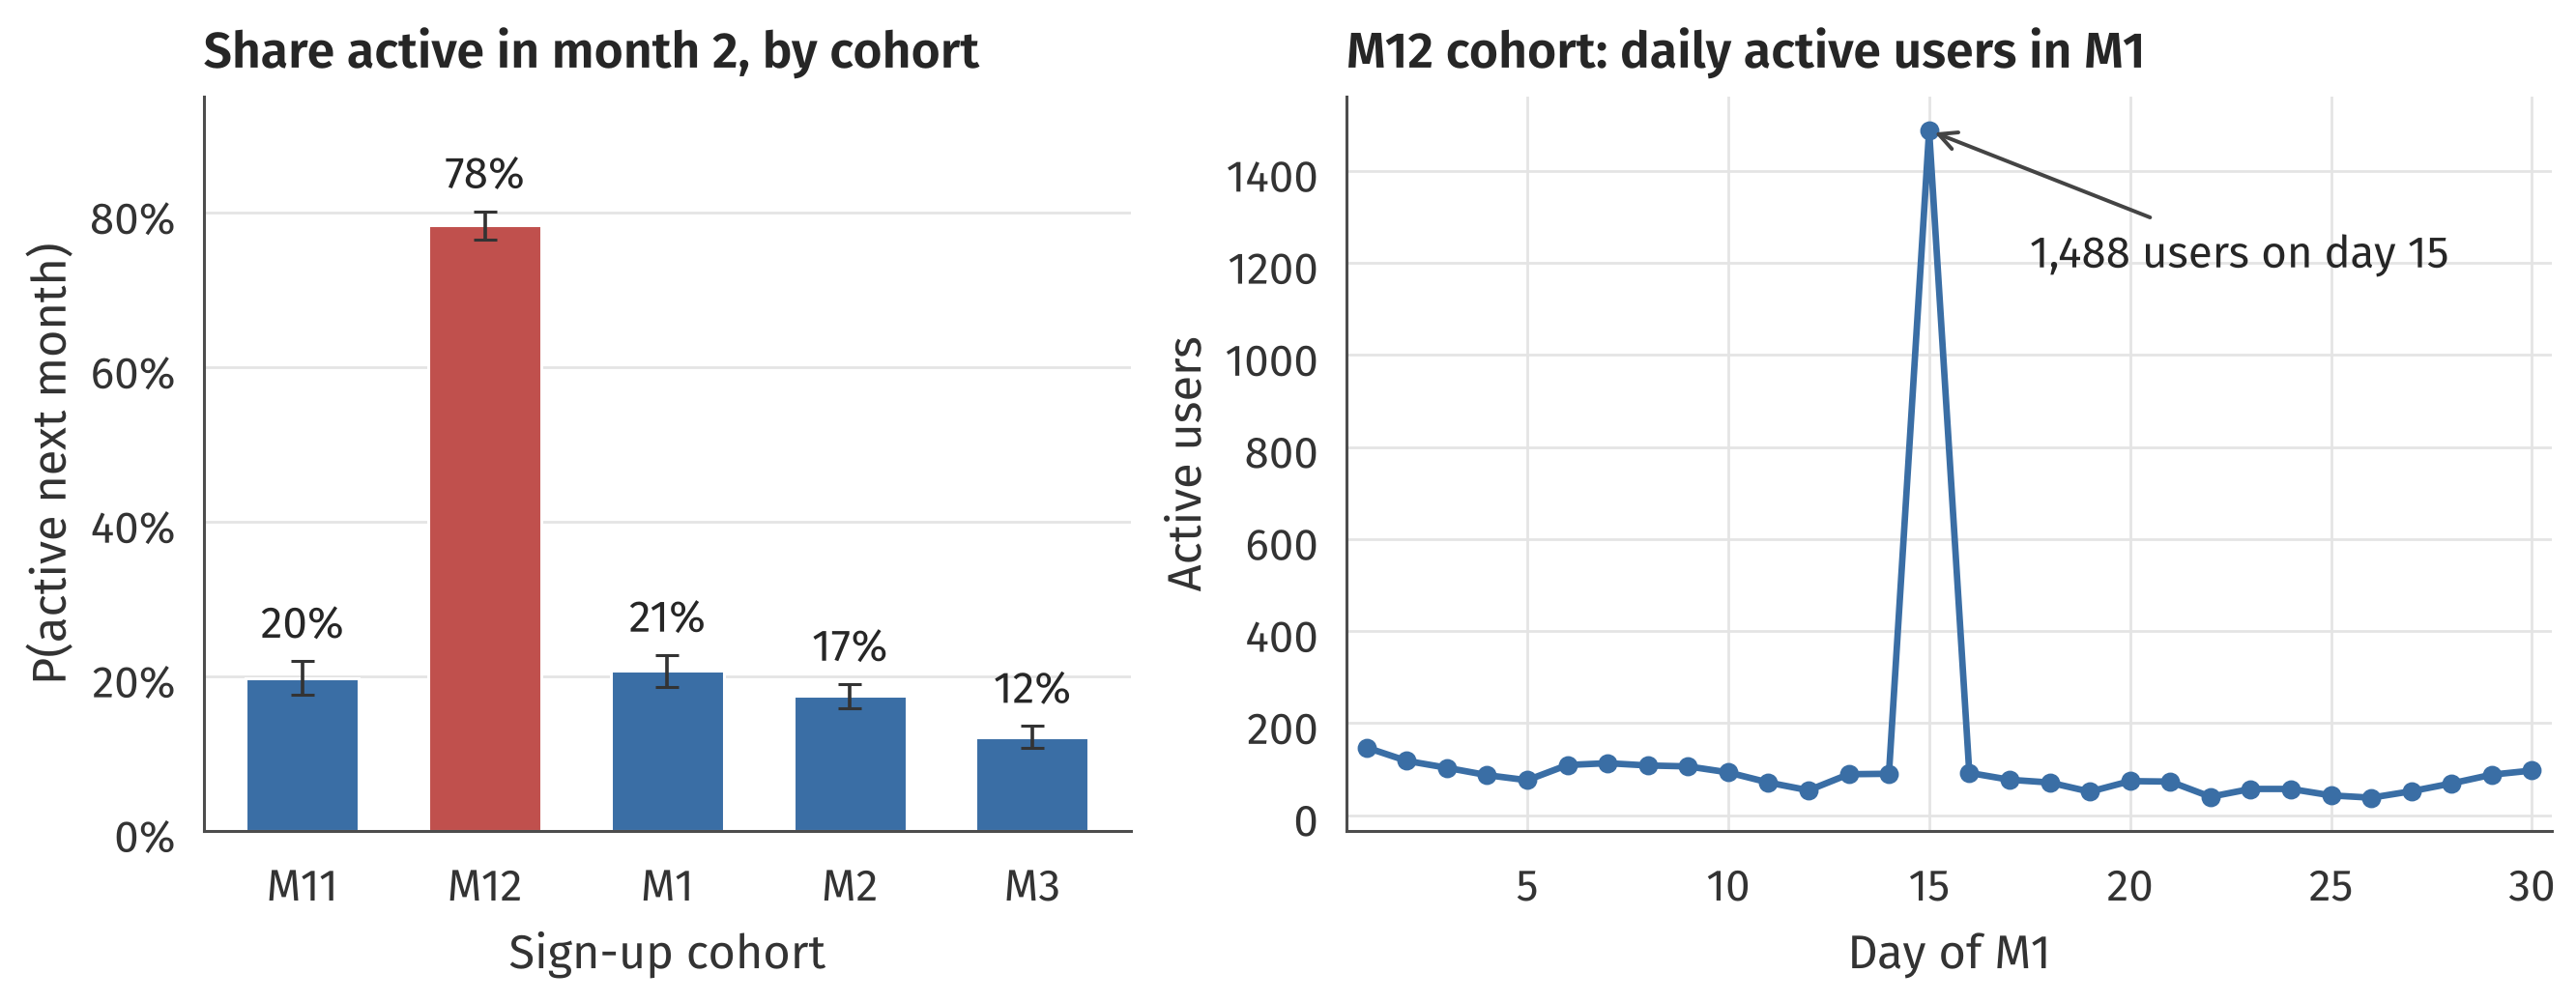
\includegraphics[width=0.97\linewidth]{fig03_cohorts}
\begin{takeaway}
\begin{itemize}
  \item M12 retains \textbf{78\,\%}: one hackathon spike ($\approx$1\,500 users on one day)
  \item $\Rightarrow$ \textbf{time-based validation}; test \textbf{dropping M12} from training; add \texttt{joined\_hackathon}
\end{itemize}
\end{takeaway}
\src{Notebook \S3.1}
\end{frame}

\begin{frame}{EDA 2: first-month engagement and behaviour}
\begin{columns}[c]
\column{0.73\textwidth}
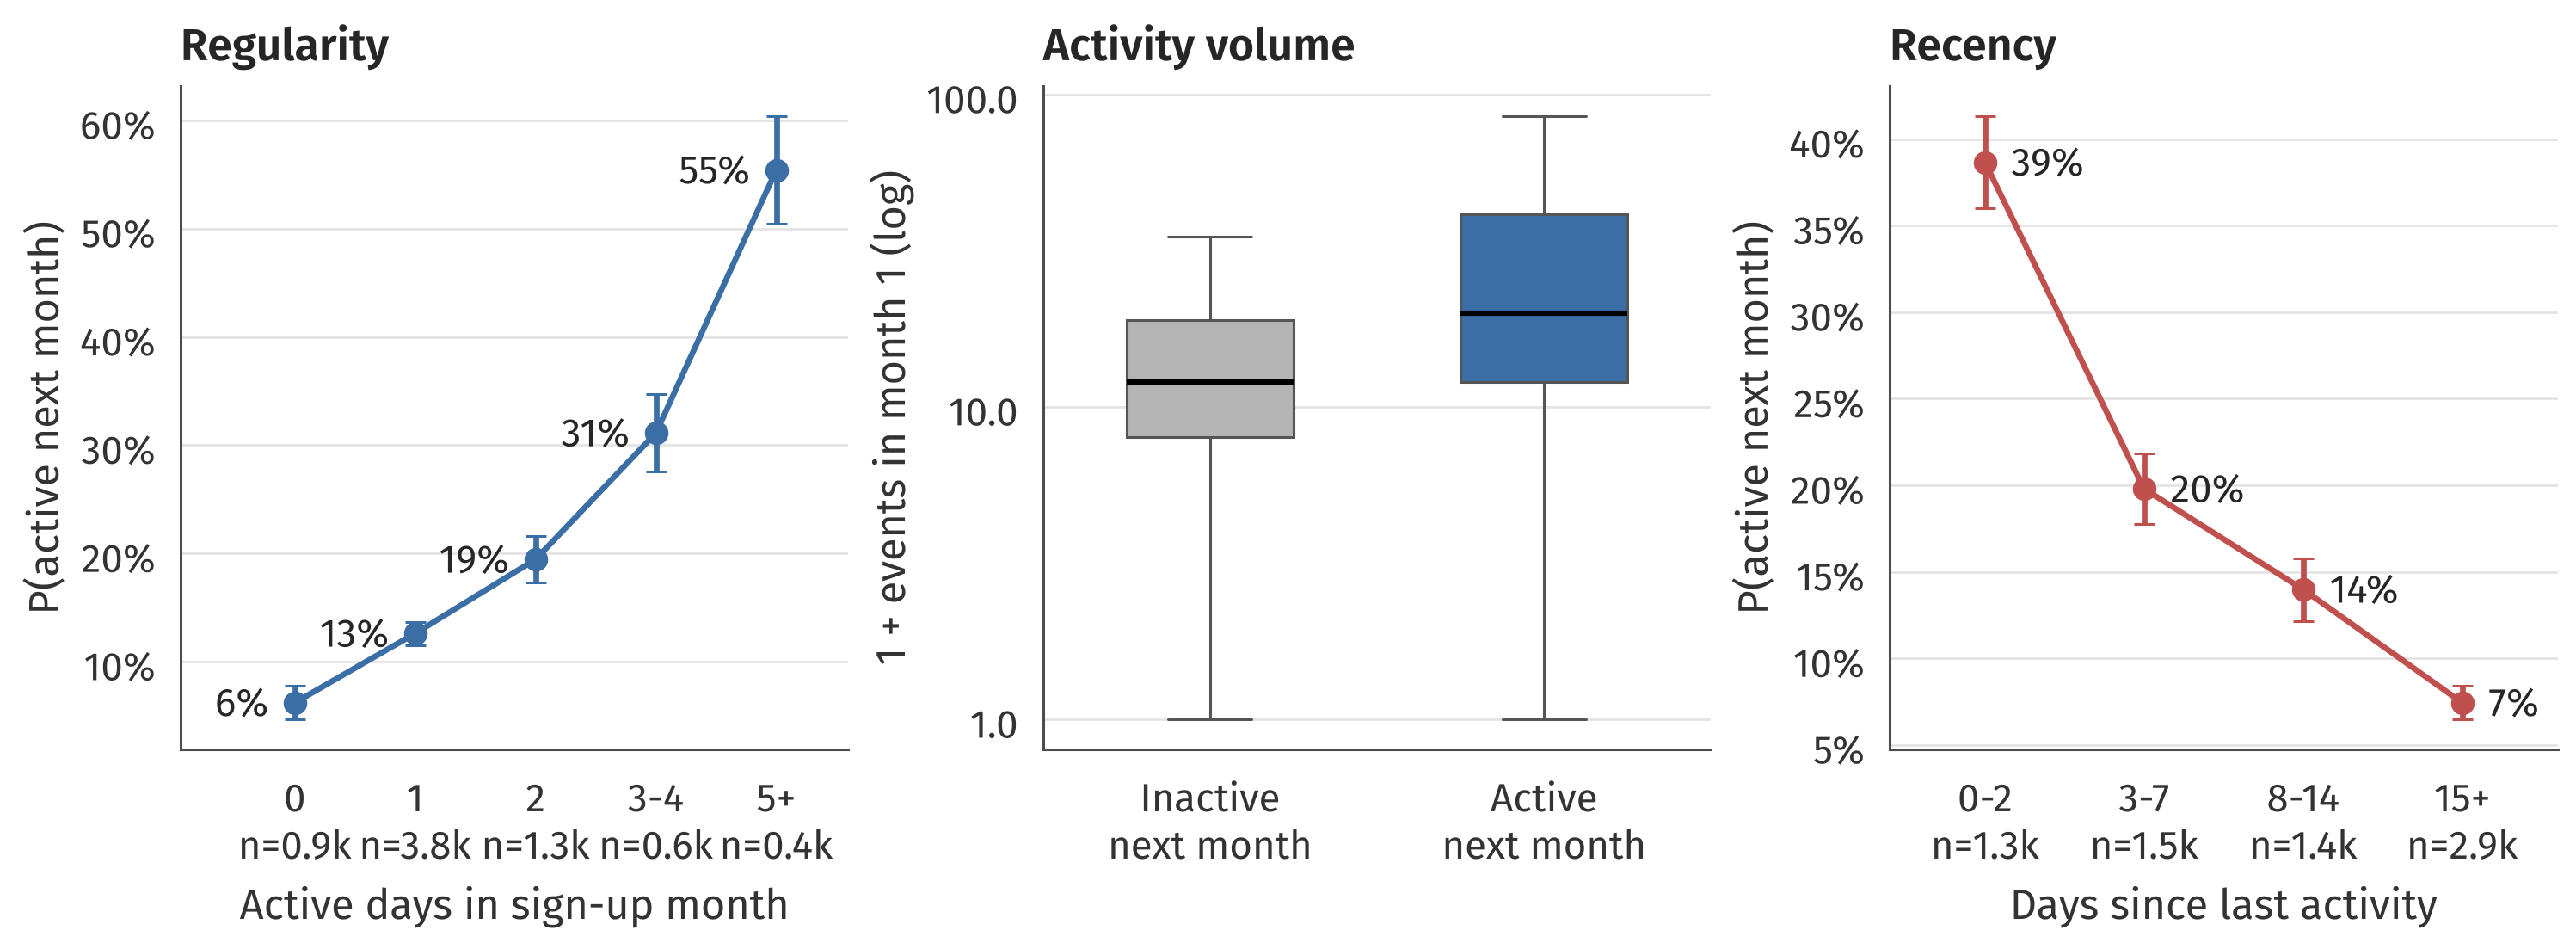
\includegraphics[width=\linewidth,height=0.405\textheight,keepaspectratio]{fig04_engagement}\\[1pt]
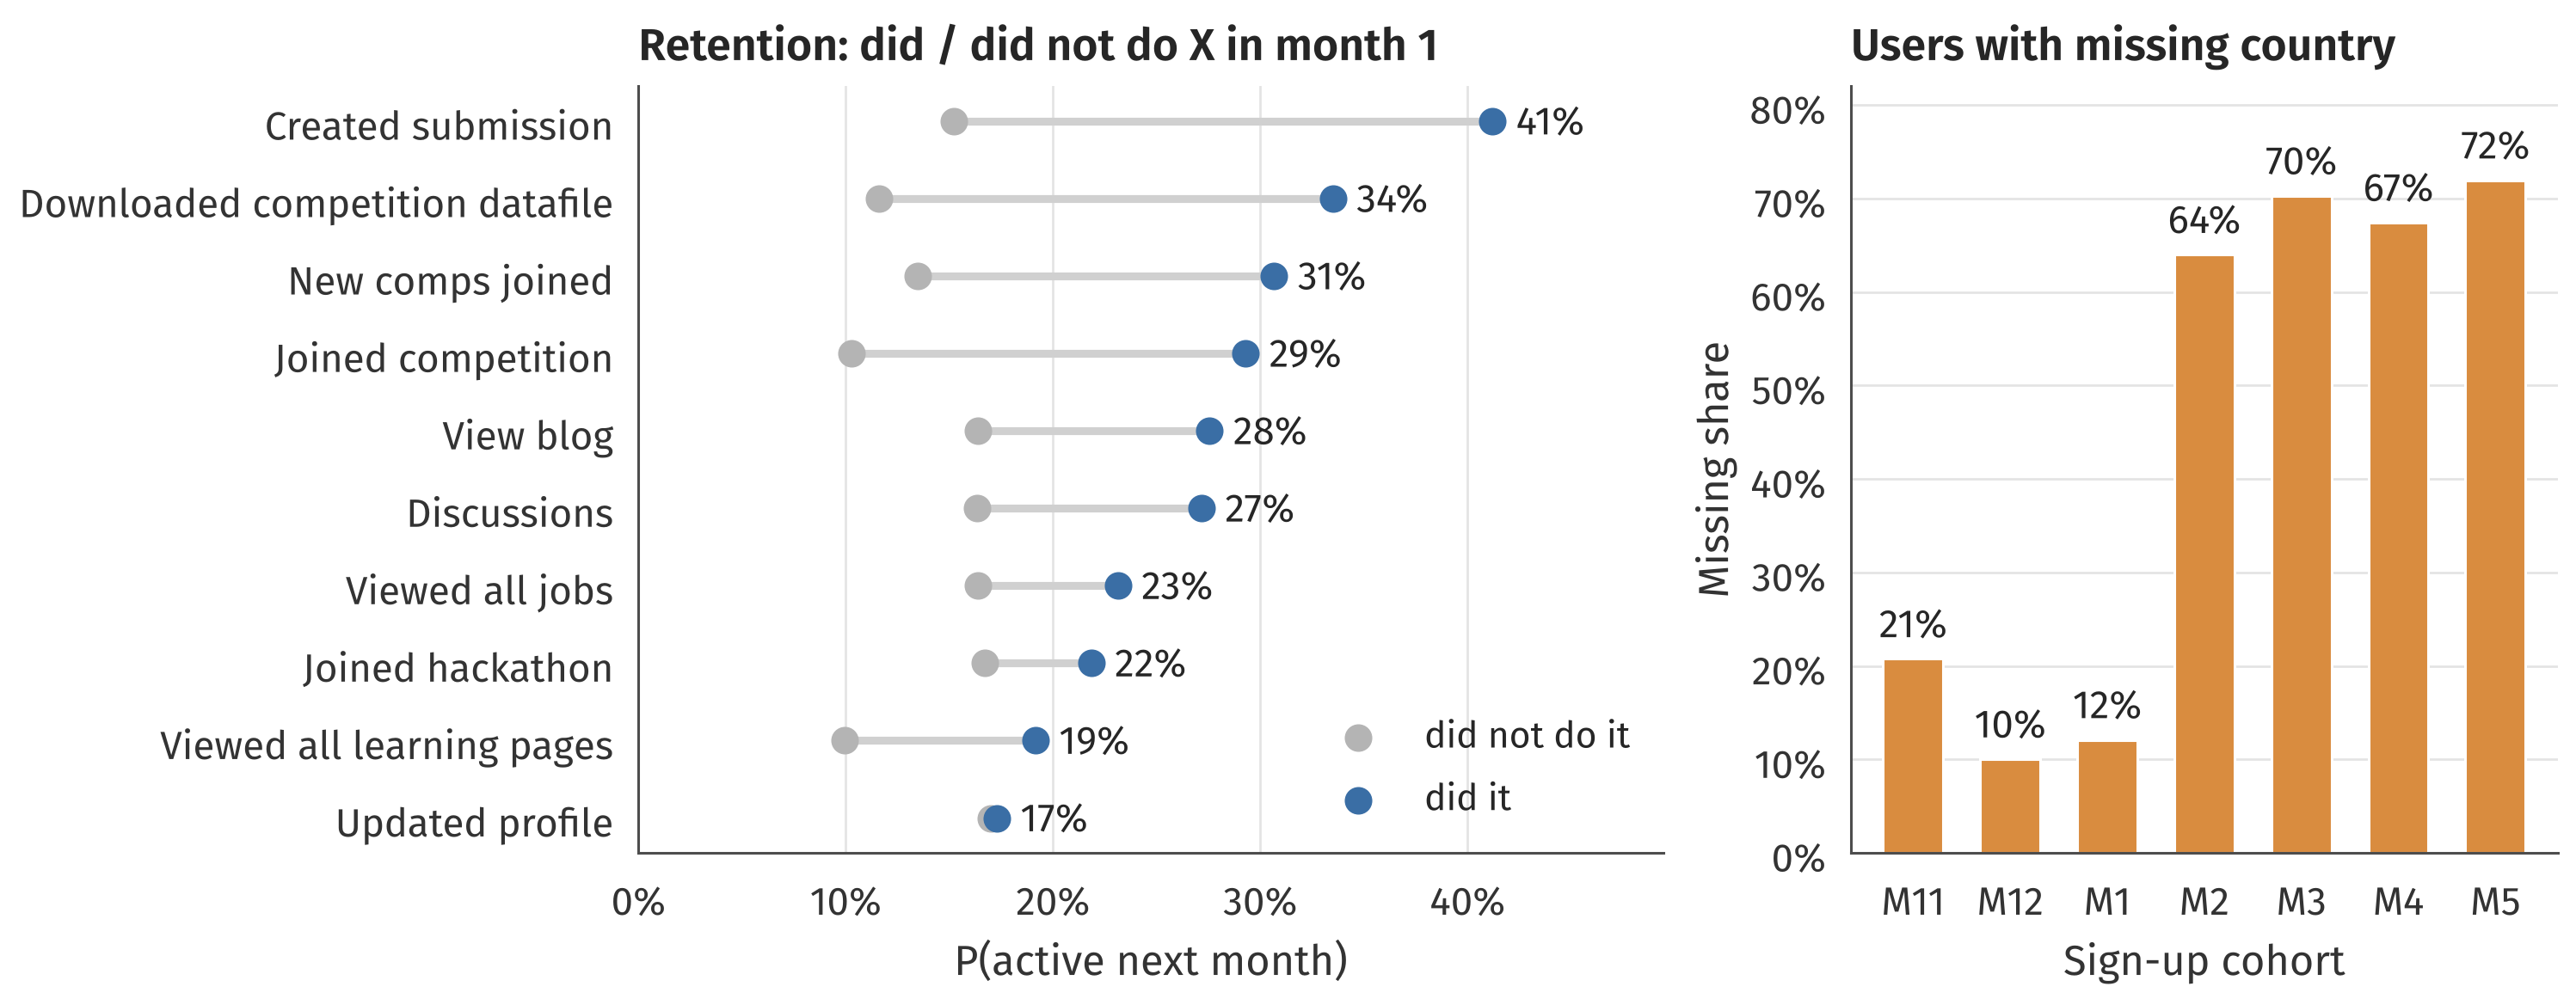
\includegraphics[width=\linewidth,height=0.405\textheight,keepaspectratio]{fig05_behaviour}
\column{0.25\textwidth}
\footnotesize
\begin{itemize}\setlength{\itemsep}{3pt}
  \item Active days: 6\,\% $\to$ 55\,\% return
  \item Seen in last 2 days: 39\,\% vs 7\,\%
  \item Submitting / downloading $\gg$ reading blogs
  \item Country missing jumps in M2 (form change) $\Rightarrow$ test \textbf{dropping country}
  \item Skewed, collinear counts $\Rightarrow$ log + L2 logistic, trees
\end{itemize}
\end{columns}
\src{Notebook \S3.2--3.3}
\end{frame}

%================================================================
\section{Validation, metric and models}

\begin{frame}{Cross-validation and metric \rubric{CV, metric, models}}
\begin{columns}[c]
\column{0.5\textwidth}
\begin{card}{Forward chaining by cohort}
\begin{tabular}{lll}\toprule
Split & Train & Validate\\\midrule
Fold 1 & M11 (+M12) & M1\\
Fold 2 & M11 (+M12), M1 & M2\\
\textbf{Hold-out} & all above & \textbf{M3}\\\bottomrule
\end{tabular}
\end{card}
\begin{takeaway}
\textbf{Metric}: F1 of the positive class (competition metric; accuracy useless at 12\,\% positives).
Model selection by \textbf{PR-AUC}; threshold tuned on out-of-fold predictions.
\end{takeaway}
\column{0.48\textwidth}
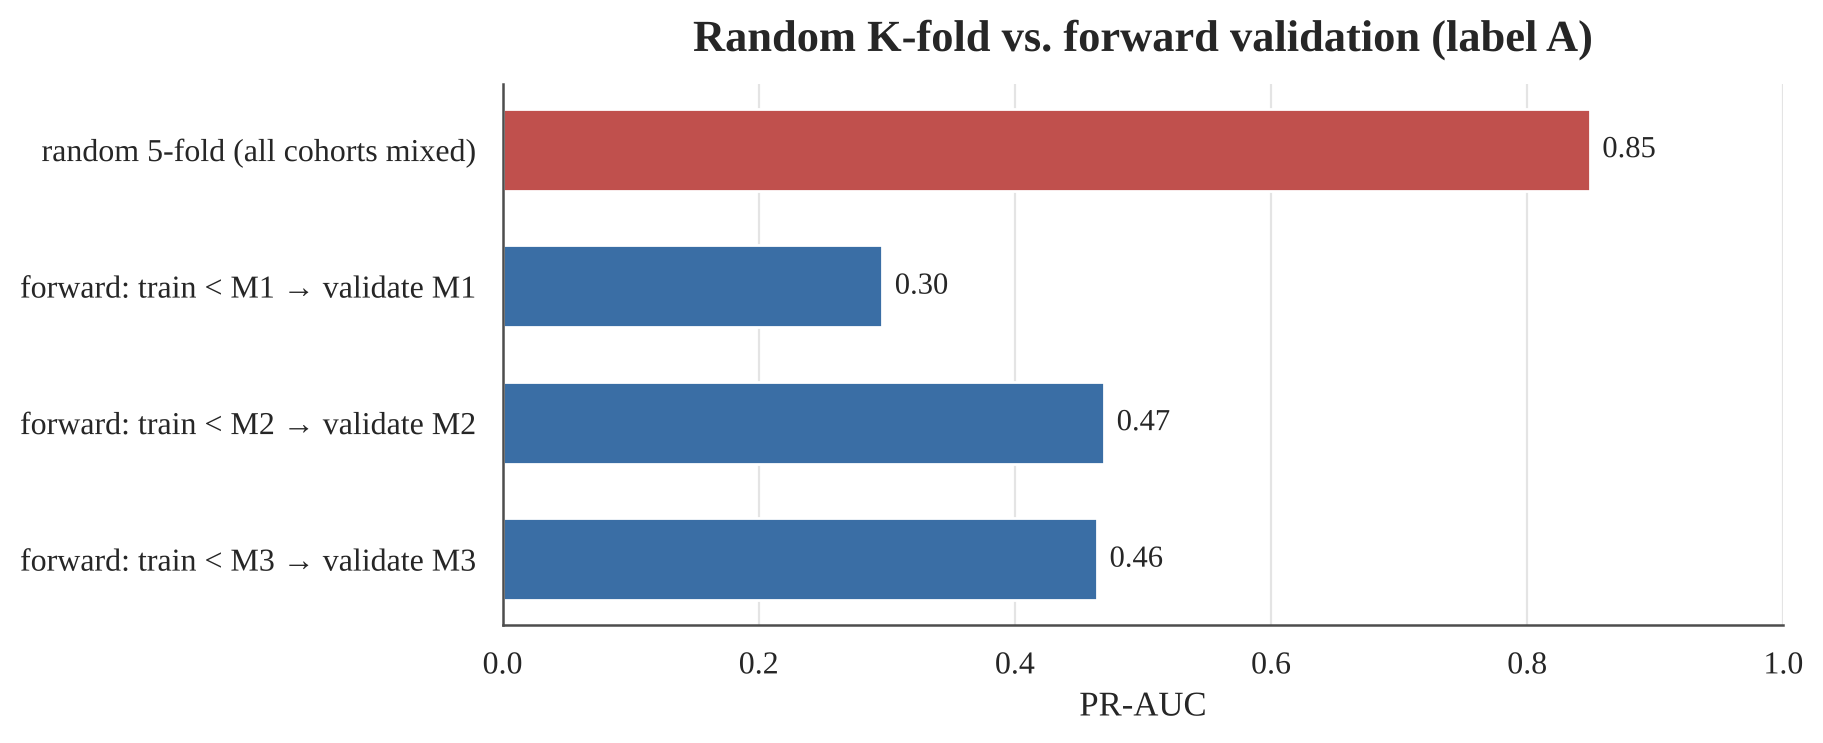
\includegraphics[width=\linewidth]{fig07_kfold}\\
\small Random K-fold reports $\sim$2$\times$ higher PR-AUC because it leaks cohort information.
\end{columns}
\src{Notebook \S4}
\end{frame}

\begin{frame}{Models and hyper-parameter search}
\begin{columns}[T]
\column{0.42\textwidth}
\begin{card}{Models}
\begin{itemize}
  \item \textbf{Baseline}: active on $\ge k$ days
  \item \textbf{Logistic regression} (log, L2)
  \item \textbf{Random forest}
  \item \textbf{Gradient boosting}
\end{itemize}
\end{card}
\small
\texttt{GridSearchCV} on our forward folds, crossed with: keep / drop M12, keep / drop country.
Run once per label.
\column{0.55\textwidth}
\small \textbf{\color{accent}CV PR-AUC, M12 dropped, no country}\\[4pt]
\renewcommand{\arraystretch}{1.15}
\begin{tabular}{lcc}\toprule
Model & Label A & Label B\\\midrule
\textbf{GradBoost} & \textbf{0.508} & \textbf{0.495}\\
RandomForest & 0.498 & 0.488\\
LogReg & 0.474 & 0.467\\\midrule
GradBoost, M12 kept & 0.425 & 0.392\\\bottomrule
\end{tabular}\\[8pt]
\begin{takeaway}
Dropping M12 helps every model. Both labels select \textbf{GradBoost}.
\end{takeaway}
\end{columns}
\src{Notebook \S5.1}
\end{frame}

%================================================================
\section{Results and impact}

\begin{frame}{Hold-out results on M3: label A vs.\ label B \rubric{Results}}
\begin{columns}[c]
\column{0.55\textwidth}
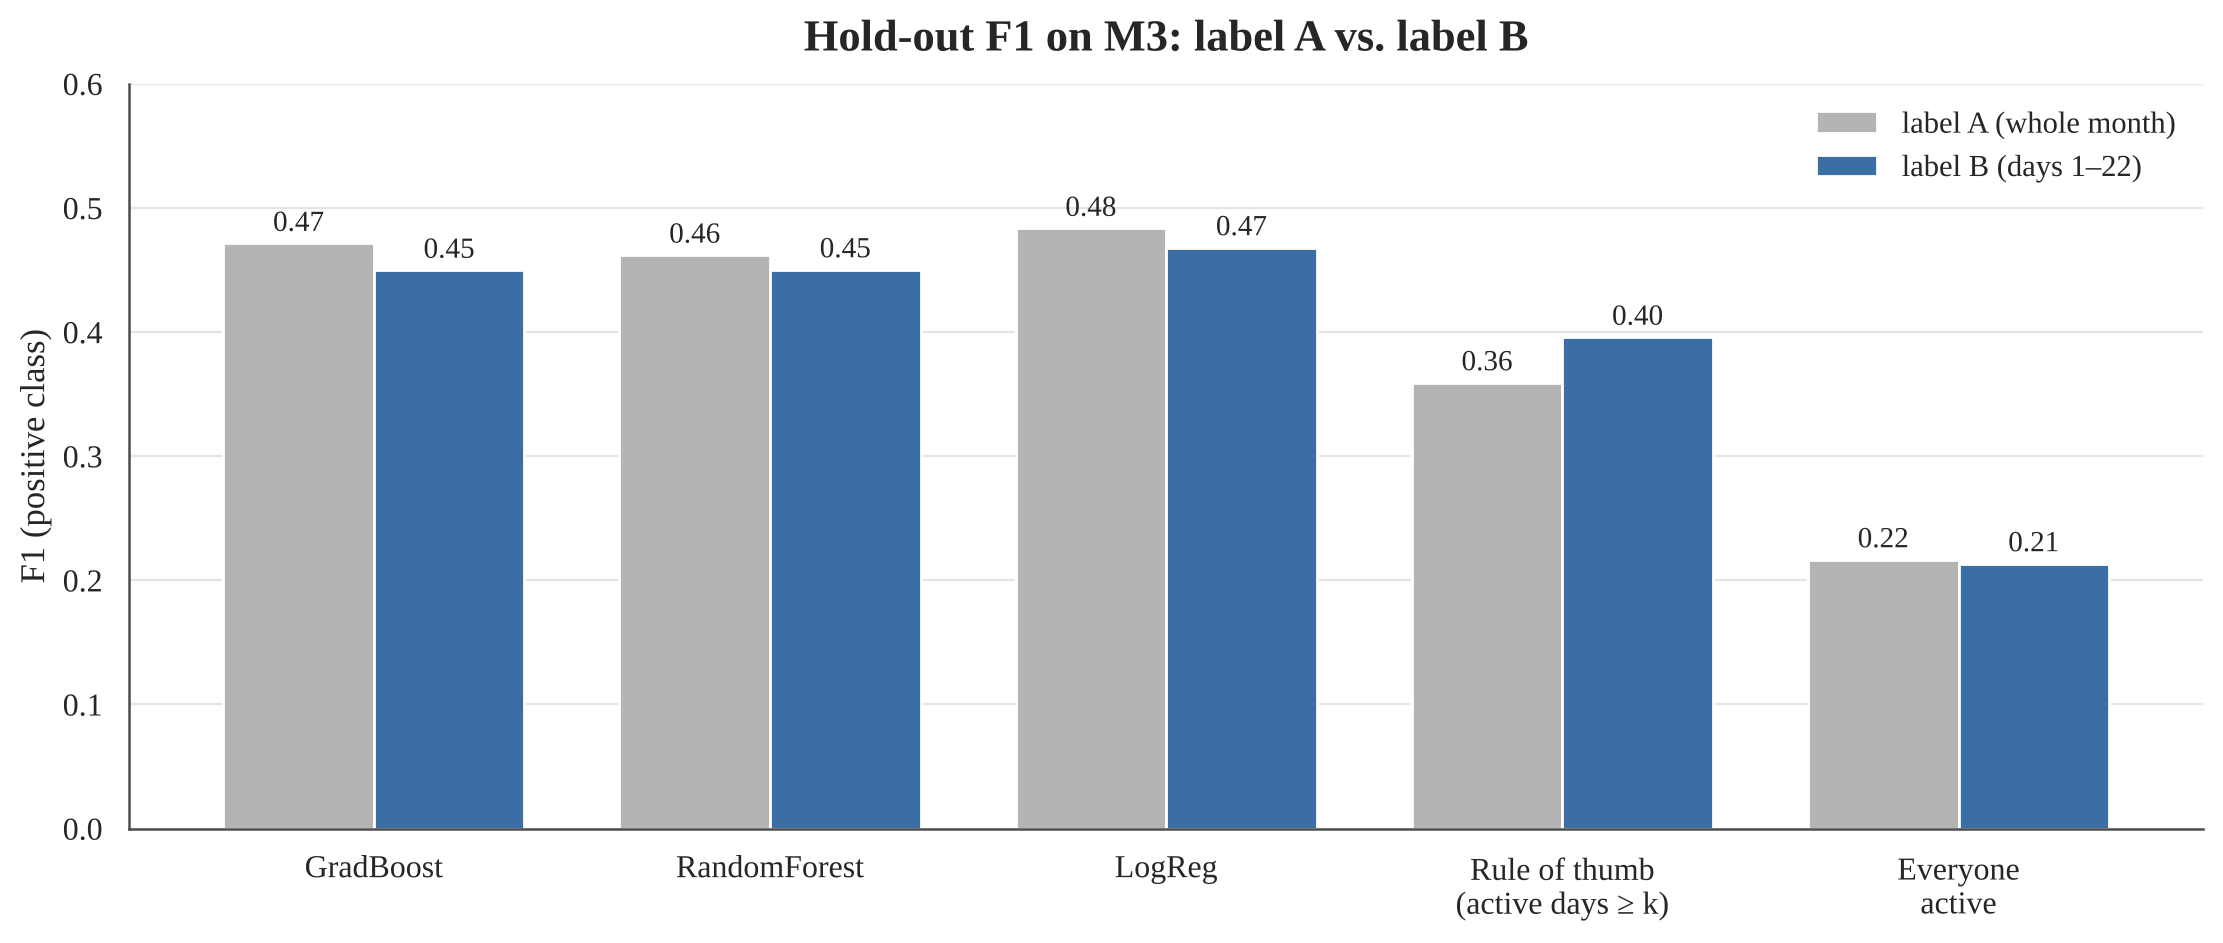
\includegraphics[width=\linewidth]{fig09_compare}
\column{0.43\textwidth}
\small
\renewcommand{\arraystretch}{1.1}
\begin{tabular}{lcc}\toprule
GradBoost on M3 & A & \textbf{B}\\\midrule
F1 & 0.47 & \textbf{0.45}\\
Precision & 0.45 & 0.44\\
Recall & 0.49 & 0.46\\
ROC-AUC & 0.83 & 0.83\\
Best rule of thumb F1 & 0.36 & 0.40\\\bottomrule
\end{tabular}\\[6pt]
\begin{takeaway}
\begin{itemize}
  \item A mixes two label definitions
  \item \textbf{B is the consistent estimate}
  \item Gap $\approx$0.02: within noise, same conclusions
\end{itemize}
\end{takeaway}
\end{columns}
\src{Notebook \S5.2}
\end{frame}

\begin{frame}{Feature importance}
\centering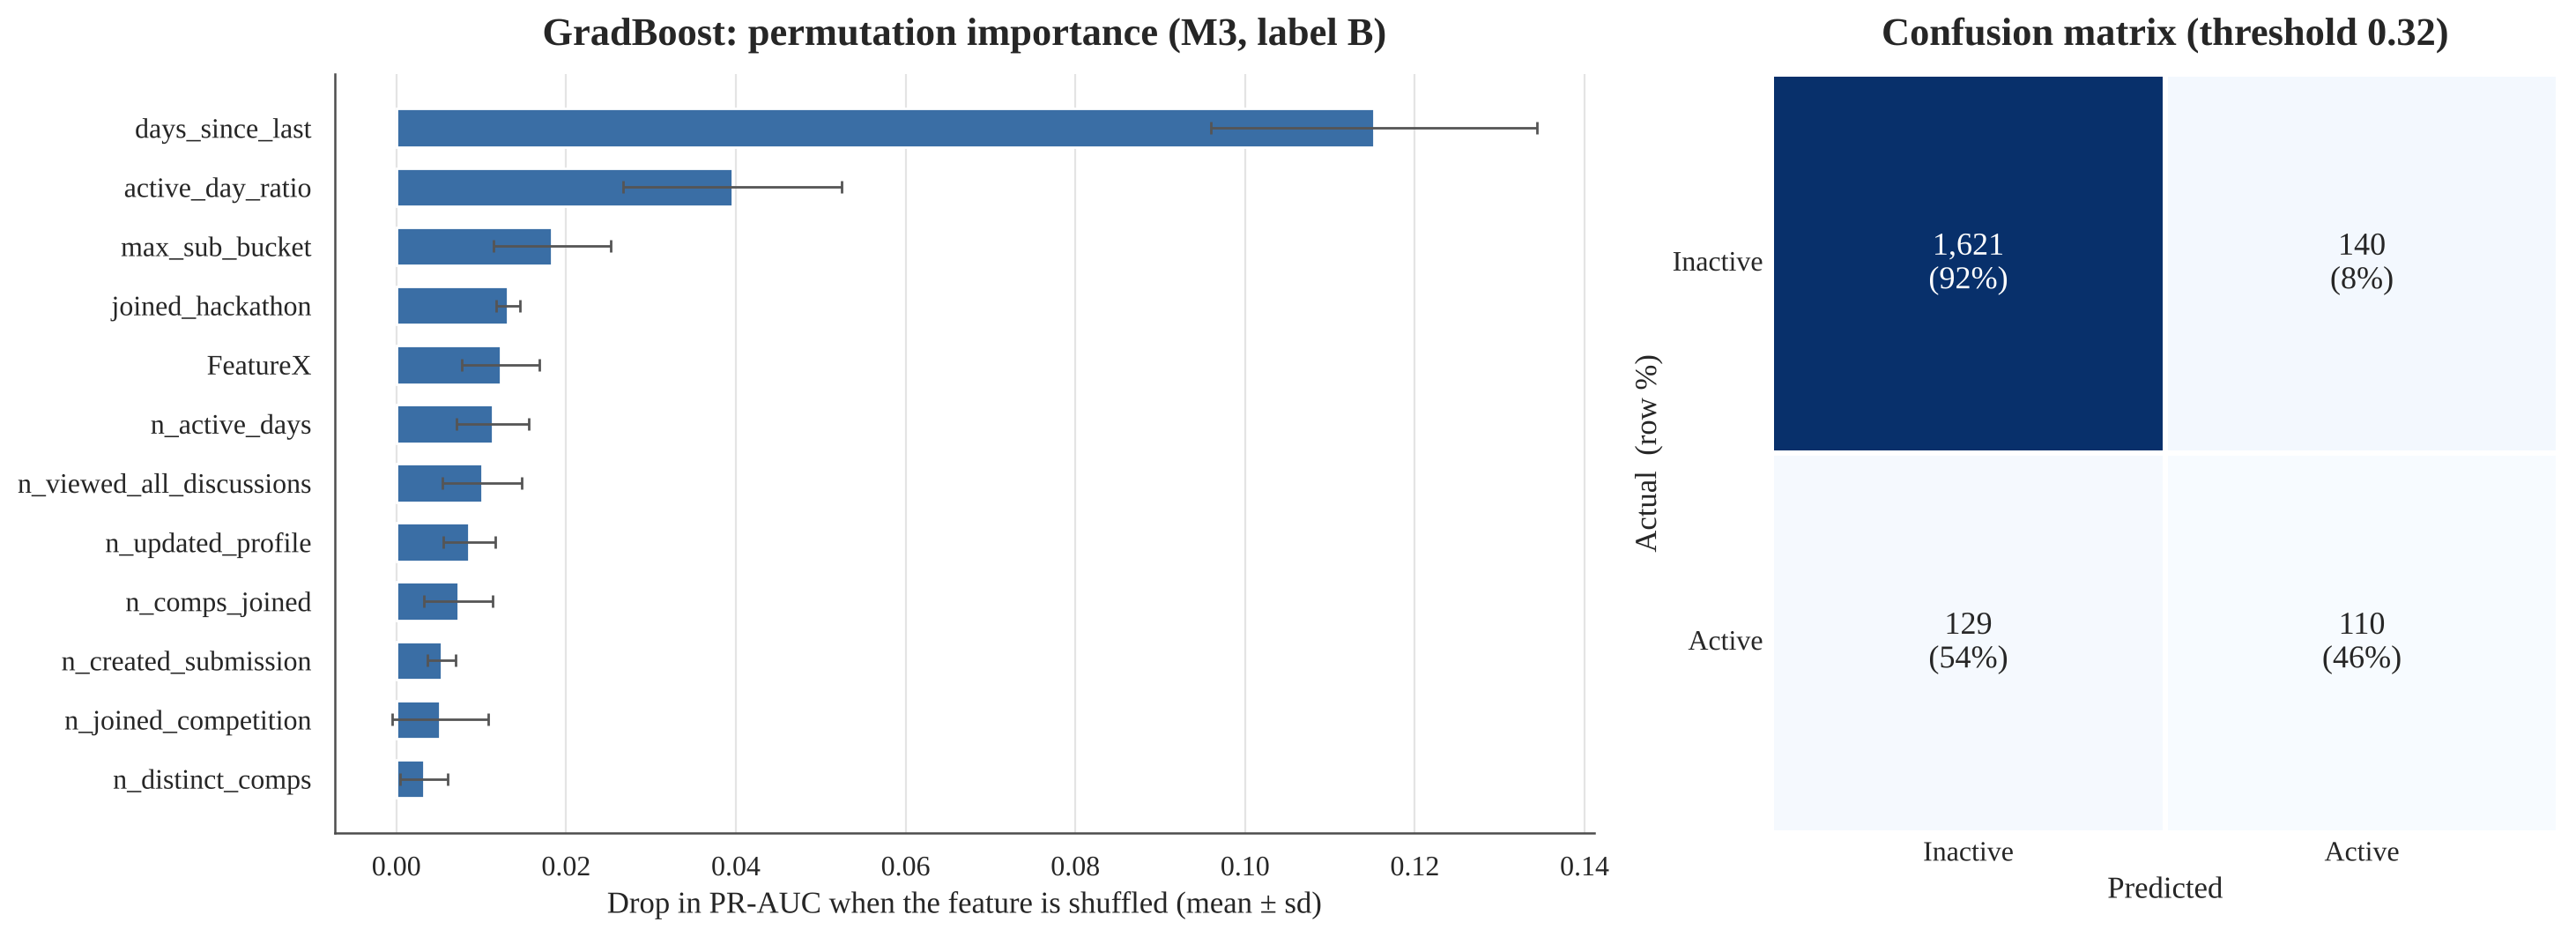
\includegraphics[width=0.88\linewidth]{fig10_drivers_B}
\begin{takeaway}
\begin{itemize}
  \item \textbf{Recency} first, then regularity and active behaviour (submissions, hackathons); demographics add little
  \item Finds 46\,\% of returners at 44\,\% precision ($\approx$3.7$\times$ the base rate)
\end{itemize}
\end{takeaway}
\src{Notebook \S5.3}
\end{frame}

\begin{frame}{Real-world impact}
\centering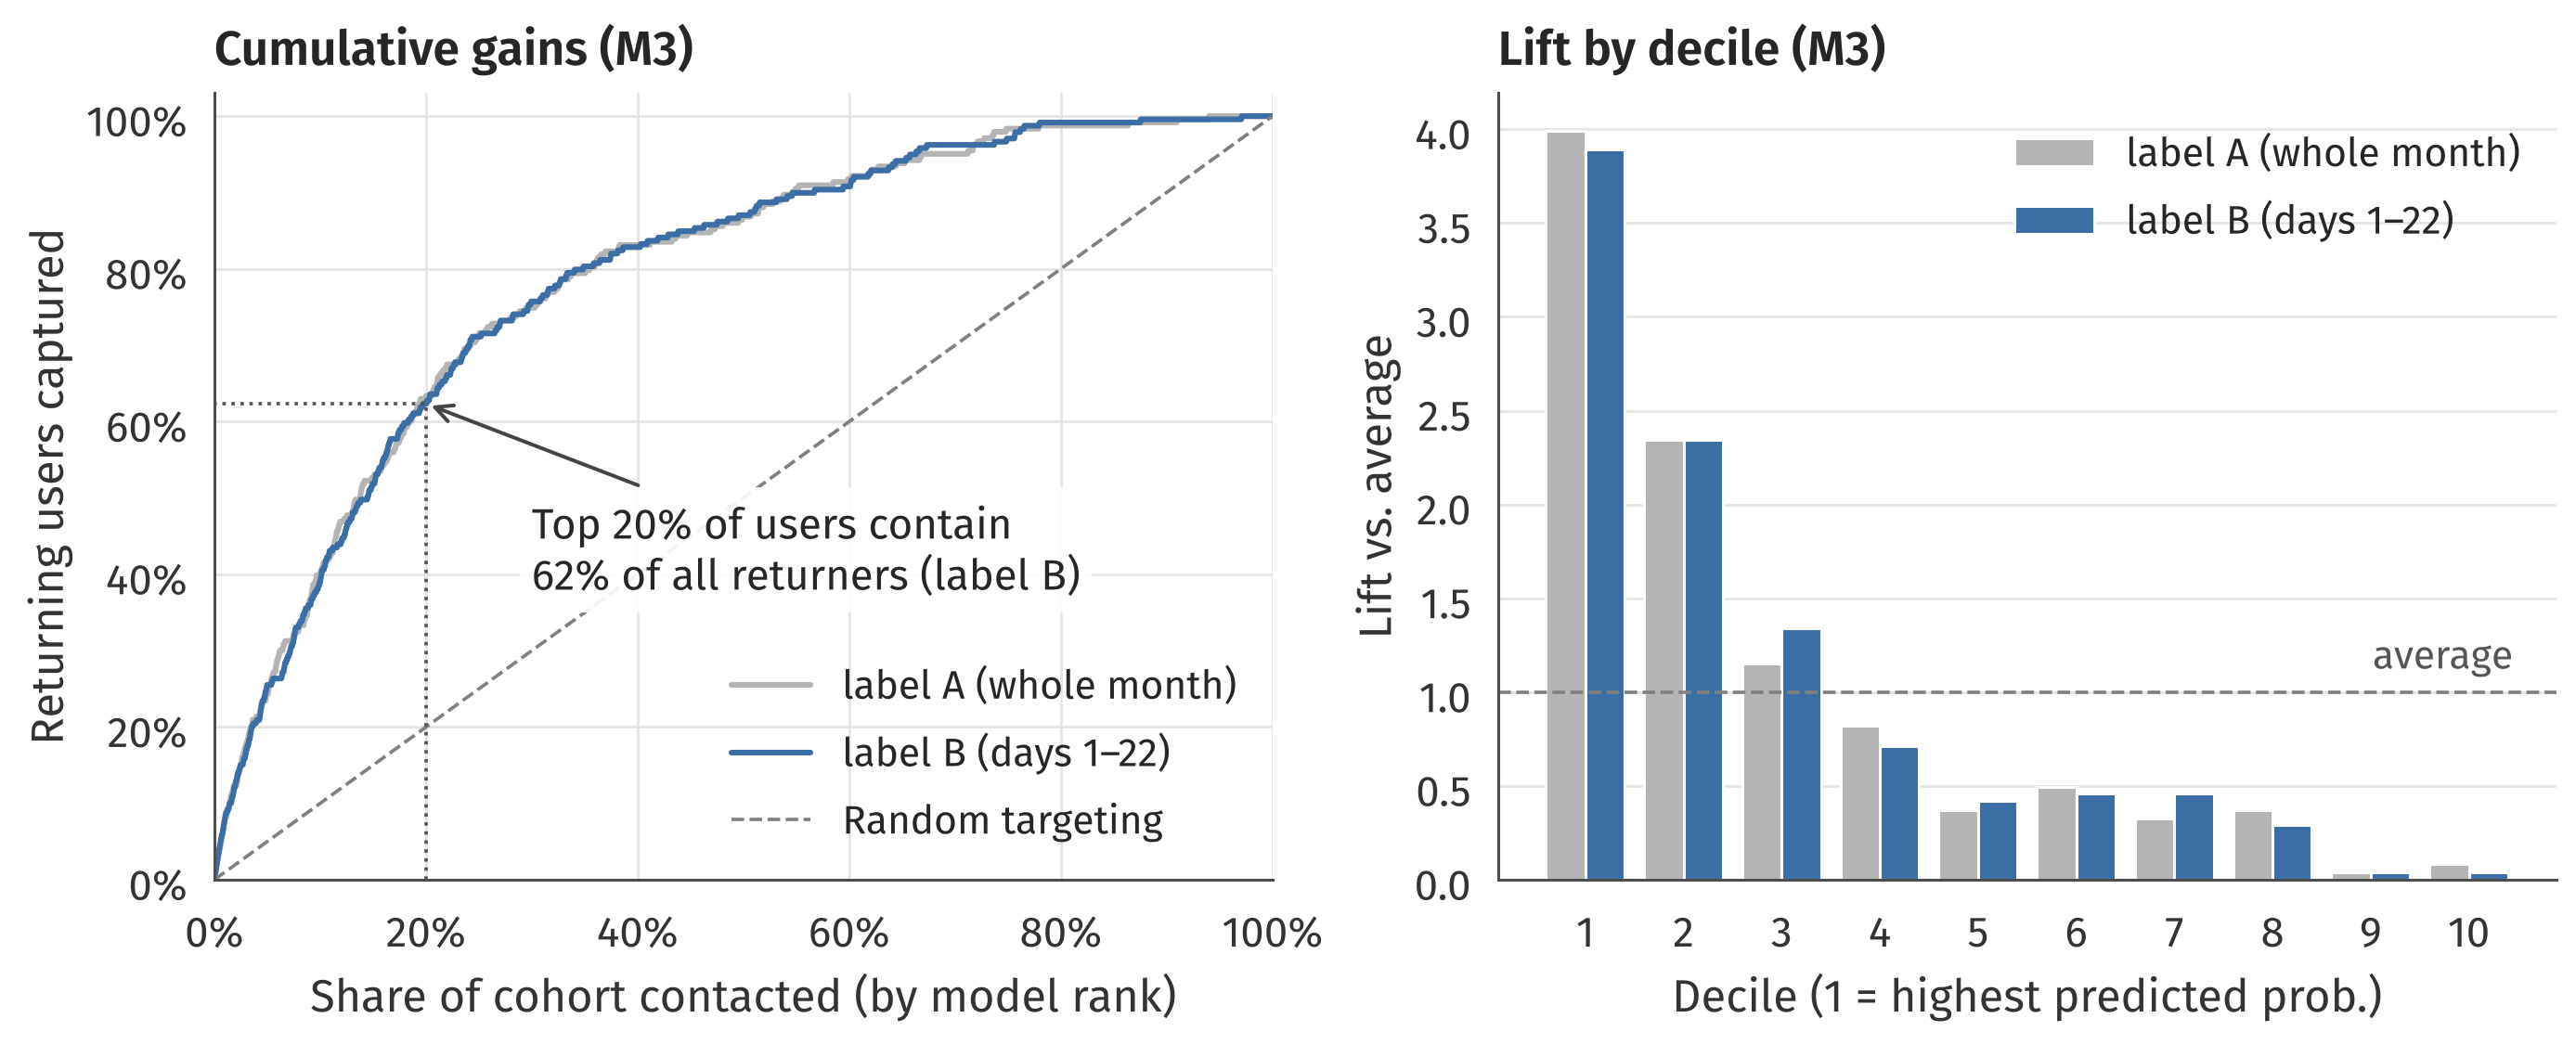
\includegraphics[width=0.8\linewidth]{fig11_gains}\\[2pt]
\raggedright
\begin{columns}[T]
\column{0.48\textwidth}
\small
\begin{itemize}
  \item Top 20\,\% of users hold \textbf{62\,\%} of returners
  \item Top decile: \textbf{$\sim$4$\times$} the average
  \item Causal effect needs an \textbf{A/B test}
\end{itemize}
\column{0.48\textwidth}
\begin{takeaway}[warn]
\textbf{Example}: 2\,000 sign-ups, 5 USD each\\
all users: 10\,000 USD\enspace$\to$\enspace middle 40\,\%: 4\,000 USD (\textbf{$-$60\,\%})
\end{takeaway}
\end{columns}
\src{Notebook \S6}
\end{frame}

\begin{frame}{Conclusions}
\begin{columns}[T]
\column{0.5\textwidth}
\begin{card}{Findings}
\begin{itemize}
  \item Recovered month order; tested on the latest cohort
  \item Fixed a label-definition inconsistency (day-22 cutoff)
  \item Recency and regularity are the main predictors; active behaviour matters more than browsing
  \item Non-stationary data: validation design mattered more than the model
\end{itemize}
\end{card}
\column{0.47\textwidth}
\begin{card}[red]{Does it solve the problem?}
\begin{itemize}
  \item \textbf{Ranking: yes}; exact classification: partly
  \item F1 0.45 (consistent) vs 0.40 rule of thumb
  \item Targeted retention $\approx$60\,\% cheaper
\end{itemize}
\end{card}
\begin{card}[grey]{Next steps}
\begin{itemize}
  \item Competition-calendar features, more cohorts, A/B test
\end{itemize}
\end{card}
\end{columns}
\src{Notebook \S7}
\end{frame}

\begin{frame}[standout]
Thank you\\[6pt]
\end{frame}

\end{document}
